\documentclass[a4paper,11pt]{jsarticle}


% 数式
\usepackage{amsmath,amsfonts,mathtools}
\usepackage{amssymb,latexsym}
\usepackage{amsthm}
\usepackage{bm}
\usepackage{physics}
% 画像
\usepackage[dvipdfmx]{graphicx}
% ローマ数字
\usepackage{otf}
% 単位
\usepackage{siunitx}
% 表
\usepackage{multirow}

\usepackage{url}

\theoremstyle{definition}
\newtheorem{thm}{定理}
\newtheorem{dfn}{定義}

\begin{document}

\title{生物進化とゲーム理論}
\author{生物物理班 齋藤駿一}
\date{\today}
\maketitle

\tableofcontents

\section{はじめに}

生物は非常によくできている.
遺伝子発現の制御や複雑な代謝経路,免疫系など,生物の教科書を少し眺めるだけでもその緻密さを実感できると思う.
では,なぜこのような仕組みが現在まで保たれてきたのだろうか.
また,現在地球上で様々な生物が見られるが,なぜ生物はそこまで多様になったのだろうか.
こうした生物に対する「なぜ」という問いに答える上で,生物進化の観点は欠かせない.
ここではこの生物進化のプロセスを説明し,さらにそれを数理的な観点で捉える試みを紹介しようと思う.

\section{生物進化の基本}
はじめに,参考文献\cite{text}に基づいて,生物の進化がどのように起こるかを(数式を使わずに)言葉で説明する.

\subsection{遺伝子の発現}
まず,生物はみなデオキシリボ核酸(DNA)という物質を持っている.
DNAはヌクレオチドと呼ばれる単位が鎖状に連なった高分子である.
ヌクレオチドは糖・リン酸・塩基の三つからなり,塩基にはアデニン(A),グアニン(G),シトシン(C),チミン(T)の4種類がある.
DNAはこの4種類の塩基の並び(塩基配列)を情報として持つ.
また,DNAは細胞分裂のタイミングに合わせて複製されるようになっている.

そしてこのDNAは転写と翻訳というステップを経て,最終的に塩基配列に応じて特定の種類のタンパク質が作られる\footnote{転写と翻訳についての詳しい話は生物の教科書に譲る.}.
タンパク質は生物体を構成し,生物の代謝や物質の輸送にも関わる.
ただし,DNAの塩基配列のうちタンパク質の設計に携わる部分は限られており,それを遺伝子と呼ぶ.
つまり,この遺伝子が生物の性質を生み出すタンパク質のもとになっている.
遺伝子からタンパク質へ至るこのような流れのことを遺伝子の発現と呼ぶ.

\subsection{突然変異と自然選択}
遺伝子の発現の話から分かるように,生物個体の性質は遺伝子に由来する.
さらに遺伝子は親から子へと受け継がれ,それによって親の形質は子の形質に受け継がれる\footnote{具体的な受け継がれ方はここでは深入りしない.}.
「蛙の子は蛙」というのは,まさしく親蛙の遺伝子が子蛙に継承されるからである.
しかし,たとえばDNAの複製の過程でミスが起こると,親と違う遺伝子が子に現れることがある\footnote{複製ミスのほかに,染色体(真核生物に見られる,DNAがヒストンと呼ばれるタンパク質に巻き付いた構造のこと)の構造変化なども要因として挙げられる.}.
このような遺伝情報の変化を突然変異といい,生まれた新しい方を変異型,もとの方を野生型という.

突然変異は生物の生存にほとんど影響しないこともあれば,決定的に関わることもある.
後者の場合,たとえば変異型が野生型の持つ重要な機能を損なっていれば,変異型は死んでしまうかほとんど子孫を残せず,その遺伝子は集団から消えていく.
一方で変異型が野生型よりも生存に有利な性質を持っていれば,むしろ野生型よりも子孫を残し,その遺伝子は集団全体に広がっていく.
このような過程を自然選択といい,「次世代に残せる遺伝子のコピー数」を適応度という.
まとめると,自然選択によって適応度の高い(子孫を多く残せる)個体のもつ遺伝子が集団全体に広がる.
このような仕組みで,世代が進むごとに集団全体を通して適応度は高くなっていく.


\section{最適化で見る進化}
以上の仕組みを考えれば,生物の集団は適応度を最大化する方向に進化していくことが分かる.
逆に言えば,現在の生物の振る舞いを「適応度の最大化」問題として導くことができると考えられる.
たとえば,植物の体には光合成を行う栄養器官(葉)と繁殖器官(花)があり,植物は成長過程でその都度どちらにどれだけ栄養を割り当てるか(どれだけ大きくするか)を決めている.
栄養器官に栄養を回せばその後に使える栄養の量を増やせるが,それだけでは繁殖器官が発達しないので子孫を残せない.
結局,適応度が最も高いのは植物の最期において繁殖器官を最大にするような割り当てと考えられる.
そこで実際にモデルを立ててそのような最適な割り当てを計算し,実際の植物の振る舞いと比較するという研究がある(詳細は参考文献\cite{text}にある.).

\section{ゲーム理論で見る進化}
こうしたアプローチが適用できるのは,適応度が「相手(同じ集団に属する他の生物)によらない」場合である.
しかし必ずしもそうとは限らない.
もし生物個体の適応度が他の生物によって変わる場合,そこには他の生物との間の駆け引きが生まれる.
このような駆け引きは,経済学に登場するゲーム理論を用いることで数理的に扱うことができる.
以降ではゲーム理論的な考えを使った考察を紹介する.

\subsection{進化ゲームの設定}
最初に,参考文献\cite{game}に基づいて,生物進化がゲーム理論における戦略形ゲームと対応づけて記述できることを見る.
ここで扱うゲームは「進化ゲーム」と呼ばれる.

まず$n$体の生物からなる集団を考え,生物個体に$i=1,2,\cdots ,n$の番号をふって区別する.
個体はいくつかの選択肢を持ち,それらを確率的に選択すると考える.
たとえば$s$,$t$という2通りの選択肢があるとき,個体は確率$p$で$s$をとり,確率$1-p$で$t$をとるという行動が許される.
このように生物個体の選択肢をとる確率が分かれば,その個体の振る舞い(戦略)が決まる.
とくに,どれか一つの選択肢だけを(確率1で)選ぶような戦略を純粋戦略といい,複数の選択肢を確率的に組み合わせた戦略を混合戦略という.
ここでは選択肢の集合は全個体に共通と考え,それを$S$とおく\footnote{つまり個体ごとの個性は選択肢ではなくその選び方(確率分布)に現れると考える.生物集団が同種の個体からなるとき,選択肢の集合$S$が種の特徴を表していると考えれば,これは自然な仮定である.}.
そして個体$i$が選択肢$s\in S$を選ぶ確率を$p_i(s)$とする.
このとき,確率分布$p_i$は個体$i$の(混合)戦略と一対一対応し,以降ではこれを``戦略$p_i$"と呼ぶことにする.

また,生物個体がとる戦略はその個体の遺伝子で決定され,途中で変えることはできないと考える.
そういう意味で,戦略とは生物個体の生まれつきの性質であるといえる.

次に,いよいよ個体間の競争を考える.
まず,生物集団内の異なる二個体$i,j$が出会うと,それらは各々の戦略に従ってそれぞれ選択肢を選ぶ.
まず簡単に,個体$i$は選択肢$s\in S$を,個体$j$は選択肢$t\in S$を確率1で繰り出す純粋戦略をとるとする.
そしてこの対戦の結果,個体$i$の利得$f_i(s,t)$と個体$j$の利得$f_j(s,t)$が決まるとする.
ここで,集団内の個体はみな対等なので
\begin{equation}
  f_i(s,t) = f_j(t,s) \eqqcolon f(s,t)
\end{equation}
が成り立つ\footnote{このようなゲームを対称であるという.}.
簡単に言えば,$f(s,t)$とは$s$と$t$が対戦したときの$s$側の利得である.
次に,個体$i,j$がそれぞれ戦略$p,q$をとる場合を考える.
このとき,この駆け引きで見込める個体$i$の期待利得(利得の期待値)は,
\begin{equation}
  F(p,q) \coloneqq \sum_{s,t\in S} p(s) q(t) f(s,t) \label{F}
\end{equation}
と書ける.
$F$は確率分布$p,q$に関して双線形な(汎)関数である.
以降では,戦略同士の対戦結果として式\eqref{F}をそのまま採用する.

ここでは,このような対戦がどの個体間でも均等に十分な回数行われると考える.
このとき個体$i=1,\cdots, n$の期待利得はその期待値
\begin{equation}
  F_i \coloneqq \frac{1}{n-1} \sum_{j=1, j\neq i}^{n} F(p_i, p_j) \label{fitness}
\end{equation}
に収束すると考えられる.
ただし,個体$k=1,\cdots,n$は戦略$p_k$をとるとした.
次世代では戦略$p_i$をとる個体の数が$F_i$倍になると考える\footnote{$F_i$倍の結果が整数とは限らないので,あくまでこれは目安である.もし次世代についても同様の議論をしたければ,各戦略$p_i$をとる個体数は$F_i$倍の結果に最も近い整数で近似するべきと考える.}.
つまり,このゲームにおける利得とは次世代にどれだけ自分と同じ戦略を残せるかに対応する.
この値$F_i$を改めて個体$i$の適応度と呼ぶ.

\subsection{進化的安定戦略}
以上の設定をもとに,適応ダイナミクスと呼ばれる過程を考える.
まず,すべての個体が同じ戦略$p$をとる生物集団を考える.
この集団の中で突然変異が起こり,戦略$q$をとる個体が現れたとする.
具体的には,戦略$p$をとる個体(野生型)と戦略$q$をとる個体(変異型)の頻度が$(1-\epsilon) : \epsilon$であると考える($\epsilon$は微小な正数とする).
つまり,集団に属する個体数を$n$として,野生型の個体数は$n(1-\epsilon)$,変異型の個体数は$n\epsilon$である.
このとき式\eqref{fitness}より,野生型の適応度$F_p$は
\begin{equation}
  F_{p} = \frac{1}{n-1} \qty[\qty{n(1-\epsilon)-1} F(p,p) + n\epsilon F(p,q)] 
\end{equation}
であり,変異型の適応度$F_q$は
\begin{equation}
  F_{q} = \frac{1}{n-1} \qty{n(1-\epsilon) F(q,p) + (n\epsilon-1) F(q,q)}
\end{equation}
である.
よって,個体数$n$が十分大きい場合を考えることにすると
\begin{equation}
  F_{p} \approx (1-\epsilon)F(p,p) + \epsilon F(p,q) ,\qquad F_{q} \approx (1-\epsilon)F(q,p) + \epsilon F(q,q) \label{fpfq}
\end{equation}
となる.
したがって,もし$F_p < F_q$なら次世代には変異型の割合が増えることになる.
一方でもし$F_p > F_q$なら次世代には変異型の割合が減ることになる.
後者の場合,野生型の戦略$p$が変異型の戦略$q$に打ち勝って,集団全体で戦略$p$が主流であり続けることになる.
このとき,戦略$p$は進化的安定戦略(ESS)であるという\footnote{ESSの存在しないゲームもある(参考文献\cite{game}).}.
ESSの厳密な定義は次のように与えられる.

\begin{dfn}[進化的安定戦略]
  \label{ess}
  戦略$p$が進化的安定戦略(evolutionarily stable strategy:ESS)であるとは,$p$とは異なる任意の戦略$q$に対してある$\epsilon_0 >0$が存在して,$0<\epsilon\le \epsilon_0$となる任意の$\epsilon$に対して,
  \begin{equation}
    (1-\epsilon)F(p,p) + \epsilon F(p,q) > (1-\epsilon)F(q,p) + \epsilon F(q,q)
  \end{equation}
  が成り立つことである.
\end{dfn}

つまり,$\epsilon$が十分小さいときに任意の変異型に打ち勝てるなら,その戦略はESSである.
しかし,実際にある戦略がESSか判定するときに毎回$\epsilon$を考えるのは面倒である.
そこで次の定理がよく用いられる.
\begin{thm}
  戦略$p$がESSであるための必要十分条件は,次の2つの性質が成り立つことである.
  \begin{enumerate}
    \item すべての戦略$q$に対して,$F(p,p) \ge F(q,p)$.
    \item $F(p,p) = F(q,p)$となる任意の戦略$q(\neq p)$に対して,$F(p,q) > F(q,q)$.
  \end{enumerate}
\end{thm}

これは関数$F$の双線形性と連続性から示せる.
証明は参考資料\cite{game}にある.

\subsection{漸進進化説}
以上で見た進化ゲームは,どのような突然変異も許して議論していた.
つまり,進化の過程は不連続に進みうると考えていた.
この考え方が間違っているわけではない\footnote{「基本的に進化は不連続に進む」という考え方を断続平衡説という.}が,その一方で漸進進化説という考え方もある.
こちらでは,効果の小さい突然変異が積み重なることで生物は連続的に進化すると考える.
漸進進化説では突然変異の可能性が制限されるので,ESSはこれまで「すべての」突然変異に耐性のある戦略と考えてきたが,もっと定義を緩くして,「ありうる」突然変異にだけ耐性があるとしても良さそうである.
また,たとえESSが存在したとしても,生物集団が実際にそこに向かって変異し続けられるとは限らない.
つまり新しく,進化の「収束性」に関わる指標が求められる.
そこで,以降では漸進進化説を採用したときの適応ダイナミクスを考える\footnote{この節での主張は参考文献\cite{text},\cite{jsmb}にあったものだが,先ほどの議論と整合するように文字や関数の定義を若干変更した.また参考文献\cite{text}では省略されていた,ESSと収束安定戦略の定義に至るまでの議論を明記した.}.

\subsection{漸進進化の定式化}
漸進進化の場合でも,式\eqref{fpfq}を導くまでの議論は同じである.
ただし,ここでは野生型と変異型の戦略$p,q$が連続的なパラメータで表せる場合を考える.
ここではごく簡単に,一般に戦略を表す確率分布$r$に対して実数$x(r)$が一対一対応すると仮定し,実数$x(r)$の変動が十分微小となる変異だけが起こりうると考える\footnote{選択肢($S$の元)が$m$個ある場合を考えると,戦略の集合は$\mathbb{R}^{m}$のうち(確率分布として)規格化条件と非負性を満たす部分集合である.たとえば$m=3$なら戦略の集合は$(1,0,0),(0,1,0),(0,0,1)$の3点を結ぶ直線に囲まれた正三角形と対応づけられる.したがって$m=2$の場合を除き,実数に対応づけられる戦略はありうる全戦略の一部にすぎない.つまりここでは,変異だけでなく生物のとりうる戦略自体も限定して考えている.}.
その仮定の下で野生型と変異型の戦略をそれぞれ
\begin{equation}
  x \coloneqq x(p),\qquad x' \coloneqq x(q)
\end{equation}
と実数で表し,これを用いて
\begin{align}
  F(x,x) \coloneqq F(p,p),\qquad &F(x,x') \coloneqq F(p,q), \\
  F(x',x) \coloneqq F(q,p),\qquad &F(x',x') \coloneqq F(q,q)
\end{align}
と書くことにする.
このとき,式\eqref{fpfq}は
\begin{equation}
  F_{x} \approx (1-\epsilon)F(x,x) + \epsilon F(x,x') ,\qquad F_{x'} \approx (1-\epsilon)F(x',x) + \epsilon F(x',x') 
\end{equation}
と書ける.
これをもとに,変異型の相対適応度を次のように定義する:
\begin{equation}
  F(x'|x) \coloneqq F_{x'} - F_{x}
\end{equation}
これが正(負)のとき,変異型は野生型を侵入することができる(できない).
また,定義より任意の戦略$x$に対して
\begin{equation}
  F(x|x) = 0 \label{F0}
\end{equation}
が成り立つ.

ここで,ある戦略$x^*$が野生型となった状態を考え,ここに戦略$x^*+\delta$が変異型として現れたとする($\delta$は実数).
このとき定義\ref{ess}をもとにすると,戦略$x^*$がESSとは,変異として可能な任意の$\delta$に対して
\begin{align}
  F(x^*+\delta|x^*) &= F(x^*+\delta | x^*) - F(x^*|x^*) \notag\\
  &= \delta\left.\frac{\partial F(x'|x)}{\partial x'}\right|_{x'=x=x^*} + \frac{\delta^2}{2}\left.\frac{\partial^2 F(x'|x)}{\partial x'^2}\right|_{x'=x=x^*} + \order{\delta^3} < 0 \label{ess1}
\end{align}
が成り立つことであるといえそうである.
ここで$\delta_0$をある微小な正数とし,$\delta$が$-\delta_0 < \delta < \delta_0$の範囲にあるような変異が許されると考える.
つまりこの範囲にある任意の$\delta$について上式が成り立つとする.
このとき,上式を$\lvert \delta \rvert$で割って$\delta \to \pm 0$それぞれの極限をとると,$\delta/\lvert\delta\rvert \to \pm 1$に注意して,
\begin{equation}
  \pm \left.\frac{\partial F(x'|x)}{\partial x'}\right|_{x'=x=x^*} \le 0 
\end{equation}
がいえる.
これがどちらの極限をとっても成り立つので,
\begin{equation}
  \left.\frac{\partial F(x'|x)}{\partial x'}\right|_{x'=x=x^*} = 0
\end{equation}
となる.
また,式\eqref{ess1}を$\delta^2$で割って$\delta \to 0$の極限をとると,今度は
\begin{equation}
  \frac{1}{2}\left.\frac{\partial^2 F(x'|x)}{\partial x'^2}\right|_{x'=x=x^*} \le 0
\end{equation}
が得られる.
ただしここで等号が成り立つとき,ESSの判定にさらに高次の項の情報が必要となって不便である.
そこでESSを次のように定義する.
\begin{dfn}[漸進進化における進化的安定戦略]
  戦略$x^*$が進化的安定戦略(ESS)であるとは,
  \begin{equation}
    \left.\frac{\partial F(x'|x)}{\partial x'}\right|_{x'=x=x^*}=0 ,\qquad \left.\frac{\partial^2 F(x'|x)}{\partial x'^2}\right|_{x'=x=x^*} < 0 
  \end{equation}
  が成り立つことである.
\end{dfn}

次に収束安定性を議論する.
戦略$x^*$が収束安定戦略であるとは,その戦略$x^*$に近い戦略をとる野生型がもっと$x^*$に近い変異型に置き換わることである.
つまり,野生型が$x^*$に十分近い戦略$x$をとるとき,$x$よりも戦略$x^*$に近い戦略$x'$をとる変異型に侵略されるということである.
そこで$x-x^*=\delta,\, x'-x=\delta'$とおくと,これは$\delta$と$\delta'$が異符号のとき$F(x'|x)>0$,$\delta$と$\delta'$が同符号のとき$F(x'|x)<0$と言い換えられる.
つまり次が成り立つ:
\begin{equation}
  \delta \delta' F(x'|x) < 0
\end{equation}
そこでこの左辺を変形すると,
\begin{align}
  \delta \delta' f(x'|x) &= \delta \delta' f(x + \delta'|x) = \delta \delta' \qty{f(x+\delta'|x) - f(x|x)}\notag\\ 
  &= \delta \delta' \qty{\delta'\left.\frac{\partial F(x'|x)}{\partial x'}\right|_{x'=x} + \order{\delta'^2}} = \delta \delta'^2 \left.\frac{\partial F(x'|x)}{\partial x'}\right|_{x'=x=x^*+\delta} + \order{\delta'^3} \notag\\
  &= \delta \delta'^2 \qty{\left.\frac{\partial F(x'|x)}{\partial x'}\right|_{x'=x=x^*} + \delta \left.\frac{\partial}{\partial x}\qty(\left.\frac{\partial F(x'|x)}{\partial x'}\right|_{x'=x}) \right|_{x=x^*}+\order{\delta'^2}} + \order{\delta^3} \notag \\
  &= \delta\delta'^2 \left.\frac{\partial F(x'|x)}{\partial x'}\right|_{x'=x=x^*} + \delta^2\delta'^2 \left.\frac{\partial}{\partial x}\qty(\left.\frac{\partial F(x'|x)}{\partial x'}\right|_{x'=x}) \right|_{x=x^*} + \order{\delta^3, \delta'^3}
\end{align}
となる.
この式についてESSのときと同様に極限を考えれば,収束安定戦略を次のように定義すれば良いことが分かる.
\begin{dfn}[収束安定戦略]
  戦略$x^*$が収束安定戦略(convergence stable strategy\footnote{後述する連続安定戦略と重複するため,ここではCSSとは略さない.})であるとは,
  \begin{equation}
    \left.\frac{\partial F(x'|x)}{\partial x'}\right|_{x'=x=x^*} = 0 ,\qquad
    \left.\frac{\partial}{\partial x}\qty(\left.\frac{\partial F(x'|x)}{\partial x'}\right|_{x'=x}) \right|_{x=x^*} < 0
  \end{equation}
  が成り立つことである.
\end{dfn}

また,ESSと収束安定戦略の定義を見比べると,両方とも
\begin{equation}
  \left.\frac{\partial F(x'|x)}{\partial x'}\right|_{x'=x=x^*} = 0
\end{equation}
が含まれる.
これが成り立つような戦略$x^*$は進化の到達点の候補であり,進化的特異点と呼ばれる.

\subsection{PIPによる可視化}
これまで,1つのパラメータで記述できる漸進進化の適応ダイナミクスについてESSと収束安定戦略を定義した.
ここではこの適応ダイナミクスを可視化し,集団内の戦略の遷移をより直観的に捉える手法を紹介する.

まず横軸に野生型の戦略$x$をとり,縦軸に変異型の戦略$x'$をとる.
次にこの2次元平面を,$F(x'|x)$の正負によって塗り分ける.
たとえば$F(x'|x)>0$の領域を黒に,$F(x'|x)<0$の領域を白に塗り分ける.
こうしてできたグラフをPIP(Pair-wise Invasibility Plot)という.
グラフの作り方から,白黒の境目では$F(x'|x)=0$が常に成り立つ.

相対適応度を表す関数$F(x'|x)$によっていろいろなPIPはあり得るが,式\eqref{F0}より,直線$x=x'$は白黒の領域の境目になり得る.
ここでは簡単のため,直線$x=x'$が常に白黒の領域の境目になる状況を考える.
また$x=x'$は変異型が存在しない状態を意味するので,PIPを読み取る上で重要である.
たとえば,最初$x=x'$上にある状態に新しく変異型が生まれ,それが侵入して集団全体に定着すると再び$x=x'$上に戻る.
これを繰り返すような適応ダイナミクスを考えると,直線$x=x'$の近傍における白黒が重要になる.
ここで,もし直線$x=x'$から少し上($+x'$)方向にずれたところが常に黒で,下($-x'$)方向にずれたところでは常に白だとすると,$x$の大きな戦略が次々と侵入し,$x$は無制限に大きくなっていく.
逆に下方向にずれたところで常に黒,上方向にずれたところでは常に白の場合は,$x$は無制限に小さくなっていく.

では,直線$x=x'$上に$F(x'|x)=0$となる別の曲線が交わり,それを境に$x=x'$の上下の状況が変わったらどうなるだろうか.
ここではそれを図\ref{fig:pip}に示した4通りの状況に分けて考える.

\begin{figure}[htbp]
  \centering
  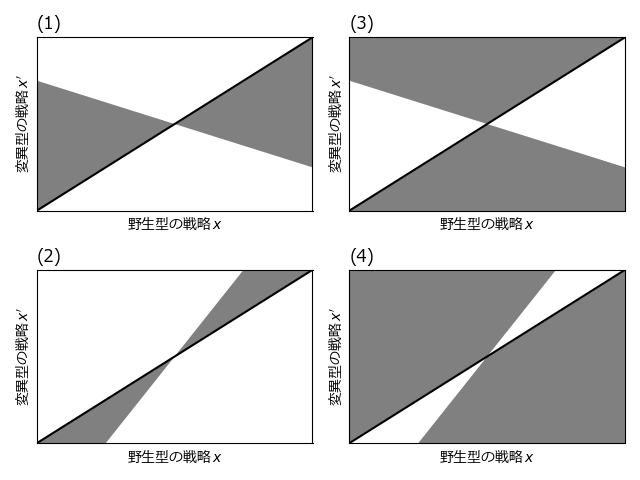
\includegraphics[width=13cm]{pip.png}
  \caption{代表的なPIP.直線$x=x'$は太線で示し,$F(x'|x)>0$の領域を灰色で,$F(x'|x)<0$の領域を白色で塗りつぶした.また2つの直線の交点の座標を$(x^*,x^*)$とする.}
  \label{fig:pip}
\end{figure}

図\ref{fig:pip}(1)の場合,戦略$x<x^*$の野生型は戦略$x'>x$の変異型に侵入され,戦略$x>x^*$の野生型は戦略$x'<x$の変異型に侵入される.
よって戦略$x^*$は収束安定戦略である.
また,$x^*$はその付近の変異型に侵入されないので,ESSでもある.
このような戦略$x^*$は連続安定戦略(continuously stable strategy:CSS)と呼ばれ,適応ダイナミクスにより実現し安定に持続する.

図\ref{fig:pip}(2)の場合,戦略$x<x^*$の野生型は戦略$x'<x$の変異型に侵入され,戦略$x<x^*$の野生型は戦略$x'>x$の変異型に侵入される.
よって戦略$x^*$は収束安定戦略ではない.
また,$x^*$はその付近の変異型に侵入されるので,ESSでもない.
このような戦略$x^*$は,適応ダイナミクスにより実現しない上に持続できない.

図\ref{fig:pip}(3)の場合,戦略$x^*$の収束性は(2)と同じであり,進化的安定性は(1)と同じである.
よって戦略$x^*$は収束安定戦略ではないがESSである.
このような戦略$x^*$は,仮に実現すれば安定に持続するが,適応ダイナミクスで実現することはない.
この状況を旧約聖書になぞらえて,戦略$x^*$をエデンの園と呼ぶこともある.

図\ref{fig:pip}(4)の場合,戦略$x^*$の収束性は(1)と同じであり,進化的安定性は(2)と同じである.
よって戦略$x^*$は収束安定戦略だがESSではない.
このような戦略$x^*$は適応ダイナミクスにより実現するものの,すぐに変異型に侵入されてしまう.
言い換えれば,$x^*$は変異型としては強いが野生型になると弱くなる戦略なのである.
これは先述した単純な「最適化」では記述できなかった状況である.
ところが集団全体が$x^*$になったときに,$x_1>x^*$となる戦略$x_1$と$x_2<x^*$となる戦略$x_2$が同時に出現することもあり得る.
このとき$x_1,x_2$は$x^*$に打ち勝ち,集団内には$x_1$と$x_2$だけが残る.
PIP図を見るとこれらは互いに侵入可能に見えるが,これは$x_1,x_2$のどちらかが大半を占めているときの図なので,両方が同じくらいの頻度のときには使えない.
そこで,この場合に新しく(局所的な)相対適応度を定義し直すと,$x_1,x_2$よりも$x^*$から遠い戦略をとる個体が侵入可能であることが分かる\cite{geritz}.
こうして戦略は$x^*$から離れる方向に二分化する.
(ただしこの相対適応度は局所的なものなので,ある程度$x^*$から離れると侵入がなくなると考えられる.)
実際にこれをもとにしたシミュレーションによって,もともと集団全体が一つの戦略をとっていたとしても二つの戦略に分裂するという現象が確認されている.
このような現象を進化的分岐といい,このような戦略$x^*$を進化的分岐点という.
この進化的分岐は,同一の環境に生息する生物の種分化(同所的種分化)に関連すると考えられている\footnote{分裂した二戦略$x_1,x_2$がそれぞれ「種」として独立するためには,$x_1$をとる個体と$x_2$をとる個体の間の交配に制限がかかることが重要であると考えられている.}.

\section{おわりに}
進化に限らず,生命現象は複雑かつ多様である.
それを単純化して数理的に解析する研究は,生命の複雑性や多様性の中に共通する原理を見いだし,見通しの良い俯瞰的な視点を与えてくれるように思う.
%またこうして生まれた視点が新たな問題を提起し,さらなる研究を駆動するだろう.
この記事で紹介したのは,そのような研究のうちとくに進化に関するものである.
内容は参考文献にあったものだが,記事にするにあたって私が素人ながら行間を埋めた.
間違いがあれば申し訳ないが,それでも読者に何か新たな視点を提供できたなら幸いである.

\begin{thebibliography}{99}
  \bibitem{text} 山内淳.『進化生態学入門---数式で見る生物進化---』.共立出版,2012.
  \bibitem{game} 岡田章.『ゲーム理論第3版』.有斐閣,2021.
  \bibitem{jsmb} 大槻久.『数理の道具箱 Adaptive Dynamics入門(4)~進化的特異点の分類とPIP~』.日本数理生物学会JSMB News Letter No.82,pp.29-34,2017.
  \bibitem{geritz} Geritz, S. A. H., Kisdi, \'E., Mesz\'ena, G. and Metz, J. A. J. Evolutionarily singular strategies and the adaptive growth and branching of the evolutionary tree. \textit{Evolutionary Ecology} \textbf{12}: 35–57, 1998. \\
  \url{https://doi.org/10.1023/A:1006554906681}
\end{thebibliography}

\end{document}